\documentclass[a4paper, 11pt]{article}

\usepackage{graphicx}
\usepackage{amsmath}
% \usepackage{amsfonts}
\usepackage{amssymb}
\usepackage{authblk}

\usepackage{tikz}
\usetikzlibrary{arrows,backgrounds,snakes,patterns}
\usetikzlibrary{shapes,arrows,chains}
\usepackage{verbatim}
\usepackage{booktabs}

\usepackage[flushleft]{threeparttable}

% Added Packages ========
\usepackage[style=apa,citestyle=authoryear]{biblatex}
\addbibresource{dl-bibliography.bib} 

\usepackage[margin=1in]{geometry} % set margin to one inch
\usepackage{float}
\usepackage{blindtext}
% Code highlighting
\usepackage{listings} 
\usepackage{color}
% \usepackage{lmodern,textcomp}
\usepackage{tgbonum}

 
\definecolor{codegreen}{rgb}{0,0.6,0}
\definecolor{codegray}{rgb}{0.5,0.5,0.5}
\definecolor{codepurple}{rgb}{0.58,0,0.82}
\definecolor{backcolour}{rgb}{0.95,0.95,0.92}

% \lstset{basicstyle=\footnotesize\ttfamily,breaklines=true}


\lstdefinestyle{mystyle}{
    backgroundcolor=\color{backcolour},   
    commentstyle=\color{codegreen},
    keywordstyle=\color{magenta},
    numberstyle=\tiny\color{codegray},
    stringstyle=\color{codepurple},
    basicstyle=\footnotesize\ttfamily,
    breakatwhitespace=false,         
    breaklines=true,                 
    captionpos=b,                    
    keepspaces=true,                 
    numbers=left,                    
    numbersep=5pt,                  
    showspaces=false,                
    showstringspaces=false,
    showtabs=false,                  
    tabsize=2
}
 
\lstset{style=mystyle}

% 

\begin{document}

\title{Fundamentals of Neural Networks}

\author[1]{Denis Augusto Pinto Maciel}
\author[1]{Roman Pro}
\author[1]{Mahdi Bayat}

\affil[1]{Humboldt University of Berlin, Berlin, Germany}

\maketitle

\begin{abstract}
This article is a guide to help readers build a neural network from the very basics. It starts with an introduction to the concept of a neural networks concept and its early development. A step-by-step coding tutorial follows, through which relevant concepts are illustrated. Later in the post, there is also an introduction on how to build neural networks in Keras. Finally, the reader will find instructions on how to deploy the model via an API to make it accessible to anyone interested on it.
\end{abstract}

\section{Introduction}
\label{sec:intro}
As the name tells, the idea of neural networks is inspired by how neurons work in the human brain. It is, however, crucial for the readers to know that despite the original motivation of neural networks, the NN models being used today have little resemblance to what a human brain does (Warner and Misra, 1996).  In its basic form, neural networks are composed of nodes interconnected to each other in several layers. The basic form of a NN would include an input, a hidden and an output layer. The number of nodes and layers can add to the complexity and efficiency of neural networks.  

The McCulloch-Pitts model of neuron in 1943 was one of the earliest simplified version of neural networks. It consisted of a simple neuron which received a weighted sum of inputs and output either zero if the sum was smaller than a threshold or one when it was greater than the threshold. This idea is called firing and is an interesting analogy to what an actual neuron does. Later on, in the early 1960s, Rosenblatt introduced the simple perceptron model. This was a developed version of the McCulloch-Pitts with an input and output layer. However, the linear separablilty limitation (Minsky and Papert ,1969) of simple perceptron took away the research interest in neural networks for a while. In the early 1980s, the Hopfield model of content-addressable memory, however, motivated researchers in the area again and later on with the introduction of backpropagation learning algorithm, interest in neural networks research soared. Nowadays, neural nets are used in a variety of applications to tackle problems such as classification, speech and image recognition, control systems and predictions.


\section{Literature Review}
Neural networks are being alternatively used instead of the traditional statistical models to solve prediction and classification problems. According to \cite{nielsen2015neural}, the neural networks are being more efficient in providing the best solutions to problems such as speech recognition, image recognition and natural language processing. It is also proved by various researchers that the neural network model turns out to be more effective compared to other models in data classification (\cite{savchenko2013real}). \cite{gallinari1991relations} have shown analytical results which illustrate the relations between discriminant analysis and multilayer perceptrons used to solve classification problems. A similar comparison of statistical methods with neural networks has been done by \cite{cheng1994neural}. According to \cite{dreiseitl2002logistic}, the neural networks and traditional statistical methods have been the most widely used models in biomedicine. \cite{warner1996understanding} also illustrated how neural nets performs as a nonparametric regression model with the power to model complex functional forms. Moreover, they argue that despite the genuine intention to develop a neural network by modeling the human brain, the current neural networks  have little to do with what the biological neurons do. 

Despite their power to predict and classify, neural nets are prone to errors. \cite{wilamowski2009neural} warn about the number of the nodes in the hidden layers. They argue that if too many nodes are used within the layers of network, the network will be overtrained on the training pattern and can no longer recognize the new patterns. They further claim that although a larger number of nodes will give a better generalization, a small number of nodes will provide better approximation for the new patterns. \cite{dreiseitl2002logistic} claims that it is enough to have one hidden layer to classify most data sets. However, when it comes to the number of nodes in the hidden layers, they opt for empirical results by cross-validation or bootstrapping. \cite{hansen1990neural} implements the tool of cross-validation to optimize the neural network parameters.

Cross-validation refers to the process of evaluating the performance of neural network by using a fraction of the dataset in training against the rest of the dataset and ultimately measuring the capacity of the network in order to make a generalization (\cite{hansen1990neural}). \cite{toussaint1974bibliography} defines cross-validation as a standard tool to decide among different parametrized choices for a dataset estimated using the traditional statistical methods. However, \cite{rumelhart1985learning} assert that the standard way to train a neural network is to train on the whole dataset in order to minimize the aggregate error of misclassification in the dataset. \cite{srivastava2014dropout} introduced the dropout technique to tackle the overfitting problem when the number of parameters is large. The technique is to randomly drop nodes with their connections from the network throughout the training process which will result in much lower co-adaption of the nodes.

\cite{ruder2016overview} gives a gentle comparison of different variants of gradient descent, the most commonly used optimizer for the neural networks. In his paper, he compares the batch gradient descent, stochastic gradient descent and the mini-batch gradient descent. The batch gradient descent is used to update the parameters for the entire training data. It is slow and cannot estimate the gradient for new observations during the training.  However, Ruder argues that it converges to the global minimum of the cost function if the surface is convex and converges to the local minimum for non-convex surfaces. The stochastic gradient descent, in contrast, estimates the gradient for a single randomly-selected observation in the training dataset in each iteration (\cite{bottou2012stochastic}). Bottou also claims that the stochastic gradient descent is able to estimate the gradient for the new observations during the training as opposed to the batch gradient descent. He concludes that whenever time is an issue and the data is abundant (\cite{bottou2010large}), use the stochastic gradient descent. There is a trade-off between the time of parameter update and its accuracy (\cite{ruder2016overview}). The third variant of gradient descent is the mini-batch gradient descent which estimates parameters for every mini-batch of the training observations and falls between the stochastic gradient descent and batch gradient descent. \cite{shalev2013accelerated} state that the mini-batch has gained popularity in recent years and they introduce several popular papers such as Dekel et al 2012 , Takac et al 2013, Fercoq and Richtarik 2013 and a few more who used mini-batch as the method of choice. \cite{ruder2016overview} also states that mini-batch gradient descent is the method of choice nowadays and that the term SGD (stochastic Gradient Descent) is also used when the method is mini-batch.

It is possible that the gradient converges to a local minimum instead of a global minimum during the training process. However, there are two adjustable parameters which will help to avoid the trap of local minima (\cite{sibanda2012artificial}). \cite{riedmiller1993direct} claim that the choice of learning rate will affect the convergence timing. They further argue that a small learning rate will take a considerable amount of time to converge to an acceptable value while setting the learning rate large may lead to oscillation and fail to reach the global minimum. \cite{bottou2012stochastic} advises to play with the learning rate by using a small fraction of the training dataset. Interestingly enough, \cite{ruder2016overview} shows that by dropping the learning rate slowly, the convergence of stochastic gradient descent and batch gradient descent coincide, assuring a local minimum for non-convex and a global minimum for convex surfaces. To reduce the effect of high oscillations around the local optima in order to avoid the trap of local minimum convergence, the momentum parameter is used (\cite{rumelhart1986learning}). It is believed that using momentum will stabilize the learning process and will speed up the convergence (\cite{riedmiller1993direct}).

The feedforward pass, backpropagating the error and parameters update are all key processes which make a neural network work efficiently. In what follows, the reader will find an easy step-by-step guide on how to implement all these processes from scratch, which draws inspiration from  the works of \cite{dima}, \cite{nielsen2015neural} and \cite{rashid2016make}.

\section{Neural Networks from Scratch}
\label{sec:nn-from-scratch}
\subsection{Problem Statement}

The best way to understand how neural networks work is to build one yourself from scratch. The understanding becomes even more comprehensive if there is a particular problem that can be solved using NNs. Therefore let's start our work by taking a look at Figure \ref{fig:digit-classification}.

\begin{figure}[H]
    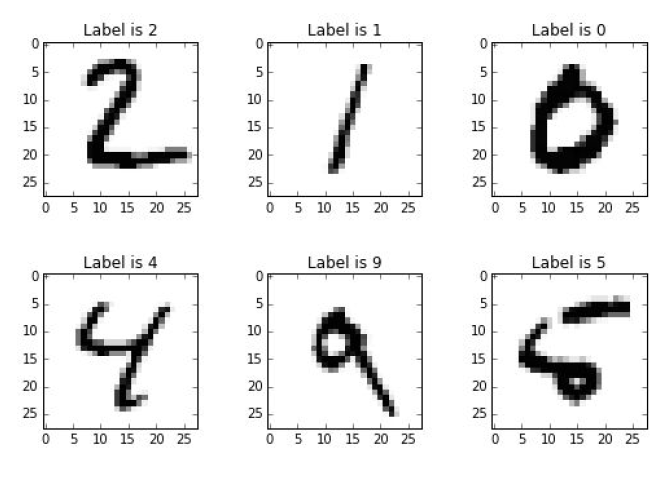
\includegraphics[width=\linewidth]{pics/problem.png}
    \caption{\label{fig:digit-classification} Digit Classification Problem}
\end{figure}

There are handwritten numbers that you want computer to correctly classify. This would be an easy task for a person but at least for a long period of time was an extremely complicated one for a machine. 

Even though the computer is faster than the human brain in numeric computations, the brain outperforms the computer in some other tasks. Many of those tasks are related to the human ability for sentience (which is a concept different from intelligence). The trick is to find a way, so that the computer could apply its numeric computation skills to solve these later tasks (at least to some degree).

The first step would be to limit the scope of the task. In our particular case the broad task of image recognition will be addressed as a classification problem - a task of giving an object a label from a given set of labels.

As we will see during the process of building our own NN, its output is based almost exclusively on application of linear algebra methods. Despite the name (which is sometimes related to the fear of artificial intelligence), neural networks in fact are much more related to statistical methods (like regression analysis or curve fitting) than to the way human brain works ??? [[Stuart Reid, 2014](http://www.turingfinance.com/misconceptions-about-neural-networks/)]. 

NNs are inspired by human brain only to certain extent. For instance the main element that makes them similar is a multilayer net structure of simple elements that are connected in some way, receiving and transmitting information. But the structure of the human brain is much more complicated, besides it is self-organizing and adaptive in contrast to the fixed manually designed architecture of a NN. Hence, there is a good reason to stop being afraid of neural networks and instead to create one ourselves.

\begin{figure}[H]
    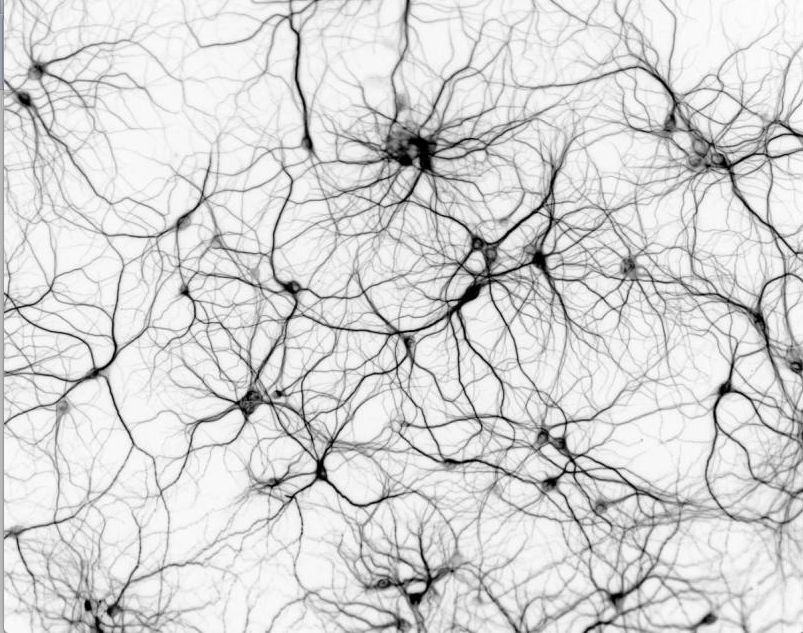
\includegraphics[width=\linewidth]{pics/neurons_net3.png}
    \caption{\label{fig:real-neurons} Brain Neurons. Source: pixabay.com}
\end{figure}


\subsection{Schematic Representation}
A complex multilayer structure that all neural networks have in common in a simplified way can be depicted using the following picture.

\begin{figure}[H]
    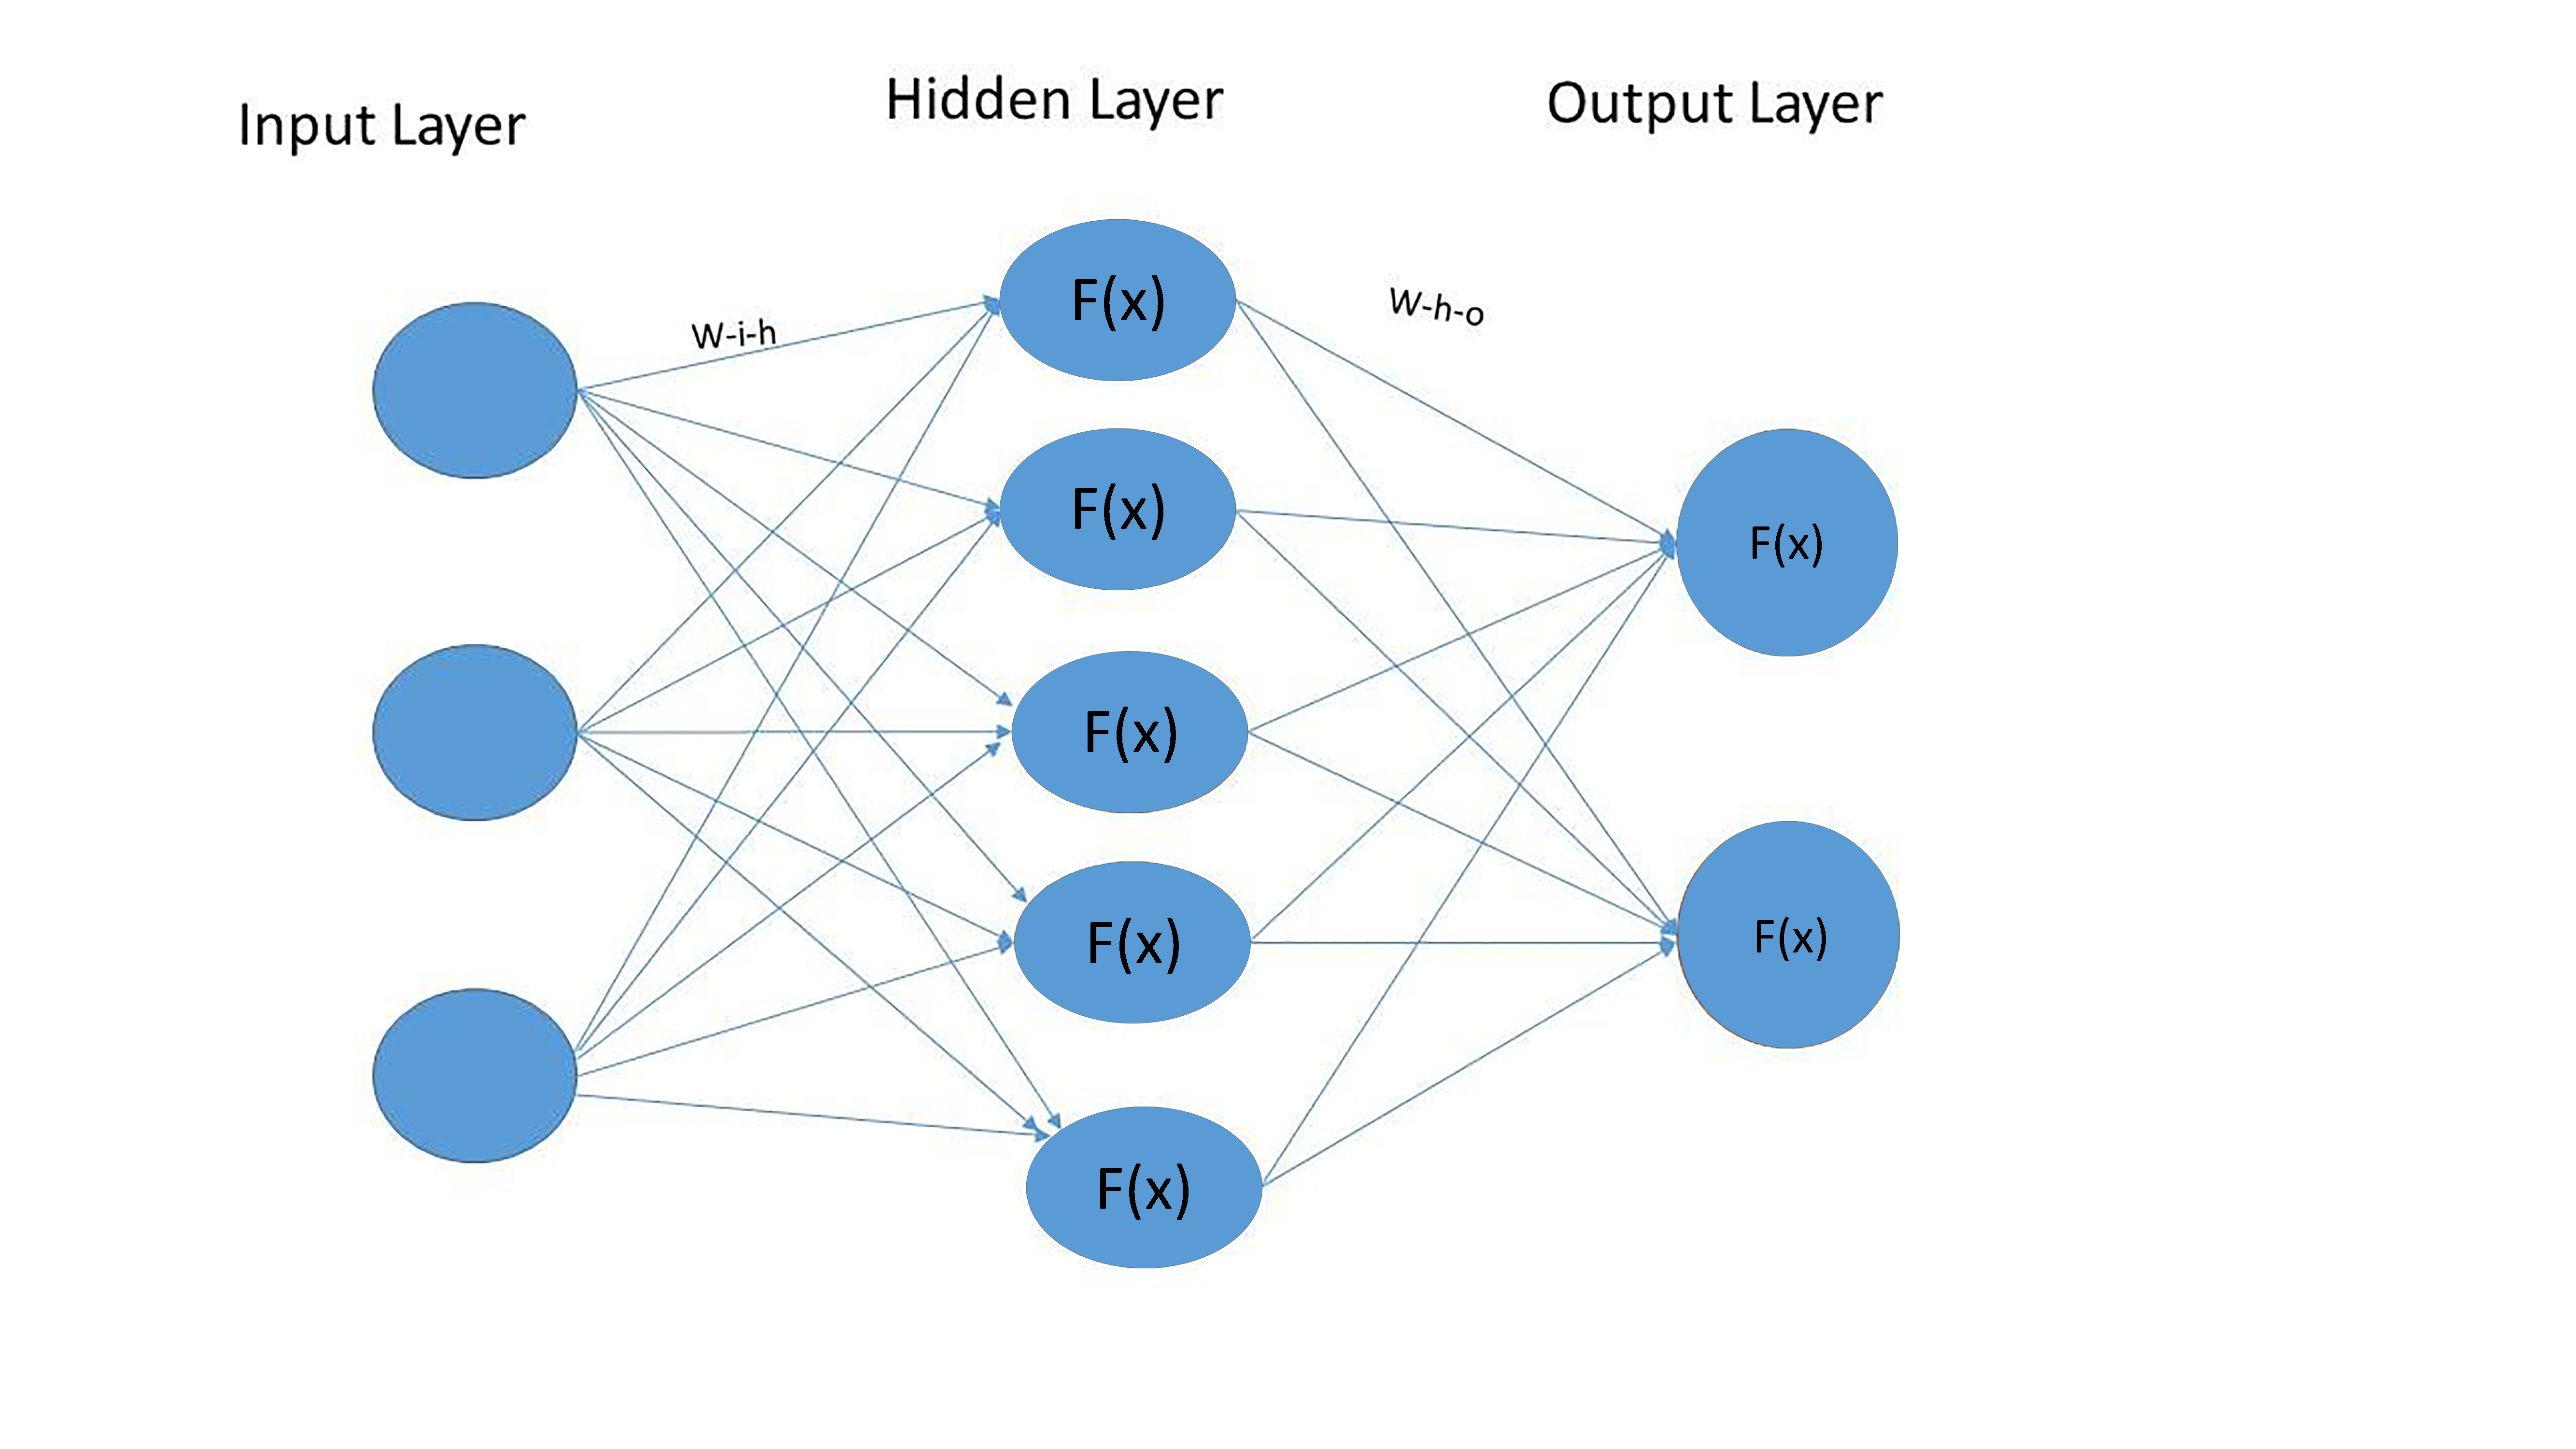
\includegraphics[width=\linewidth]{pics/neural_network1.jpg}
    \caption{\label{fig:nn-schema} Neural Network Schema}
\end{figure}

All we need in order to implement such a structure is base Python and numpy, a library for numerical computation, which we will be using to do linear algebra. 

First let's determine the elements of a neural network depicted above: nodes, layers, weights across nodes and activation functions.

\begin{itemize}
    \item \textbf{Nodes}. A node is basically a point where data points are received, processed and then transferred to the node. A node could be either an endpoint or a redistribution point or even both when iterations are done through the learning algorithm. The number of nodes to use is optional.

    \item \textbf{Layers}. A layer consists of one or several nodes. The initial layer in the network is called the input layer and it is the entry point through which the data is fed into the neural net. The middle layers are called hidden layer because the computation results of them are not directly visible to someone interacting with the neural net. In the hidden layers, which can range from one to thousands, the features are transformed and most of the structure (both linear and nonlinear) is captured. Finally, there is the final layer, from which results are output. The nodes in each layer are fully interconnected to the ones in the next and the previous layers. 


In our case we have a structure with 3 layers: input, output and one hidden layer. The number of nodes in the input  (i\_n), hidden (h\_n) and output (o\_n) layers are 3, 5 and 2 respectively. In Python, such a structure can be represented in the following way:

\begin{lstlisting}[language=Python]
    # Load the package to work with numbers
    import numpy as np
    
    # Determine the structure of the NN
    i_n = 3
    h_n = 5
    o_n = 2
\end{lstlisting}

    \item \textbf{Weights.} In order to transfer an input data point to the next layer, a predetermined number (called weight) is stored in each connection from the sender node to the receiver node. Each weight accounts for the impact between the interconnected nodes. Initially, we assign weights between nodes in neighboring layers randomly. This is needed only for the sake of initializing the structure. Later these weights will be changed in order to solve our classification problem. The weight updating will be better described in the following sections. Neural nets will have n-1 matrices of weights, where n is the number of layers in the NN. You can imagine these weight matrices sitting between two layers representing the strength of the connection between every single node of neighboring layers. Thus, each of these matrices will be of size f x p, where p is the number of nodes in the preceding layer and f is the number of nodes in the following layer.
    This becomes more clear once you check the code below that creates 2 matrices of weights: the 5x5 matrix of weights between input and hidden layers (w\_i\_h) and the 2x5 matrix of weights between hidden and output layers (w\_h\_o). Such a dimensions of matrices are necessary in order to accomplish matrix and vector multiplications that are done in the following stages.

\begin{lstlisting}[language=Python]
    # Randomly define the weights between the layers. 
    w_i_h = np.random.rand(h_n, i_n) # create an array of the given shape and populate it with random values.
    w_h_o = np.random.rand(o_n, h_n) 
    
    # Show matrices of randomly assigned weights.
    w_i_h
    # w_h_o # uncomment this line in order to see the values for w_h_o.
    # Use Cmd + / in MacOS and CTRL + / in MS Windows as a shortcut to comment/uncomment lines.
\end{lstlisting}

\begin{lstlisting}
    array([[0.63964736, 0.97236245, 0.83944375],
    [0.31439566, 0.54254369, 0.0456713 ],
    [0.93759599, 0.71292359, 0.11961199],
    [0.90587079, 0.0855728 , 0.55046849],
    [0.89559465, 0.47349711, 0.42168825]])
\end{lstlisting}

\item \textbf{Activation Function.} The remaining element of the NN's structure is an activation function - a function which transforms an input data point that it receives from the previous nodes to an output value which will be the input for the nodes in the next layer. The activation function plays an important role in the efficiency of the neural network as it accounts for non-linearity of data. 
It is to certain extent inspired by the concept of firing, which means that neurons fire or transmit information further only if the input surpasses certain threshold. The simplest activation function can be represented by a step function as on the picture below!!!. In our NN, we will use a slightly more elaborate activation function, the sigmoid function (logistic), which allows for more efficient use of the input data. An extended description of various activation functions, their benefits and disadvantages is given in sections below.

\begin{lstlisting}[language=Python]
    # Determine activation function.
    def sigmoid(x):
        # np.exp() calculates the exponential
        # of all elements in the input array.
        return 1 / (1 + np.exp(-x)) 

    # Draw activation function.
    import matplotlib.pyplot as plt
    
    # return 100 evenly spaced numbers over an interval from -10 to 10.
    x = np.linspace(-10, 10, 100) 
    # plot sigmoid function for sampled values.
    plt.plot(x, sigmoid(x)) 
    plt.show()
\end{lstlisting}

\end{itemize}


\subsection{Data Inspection}

By now we have collected all the elements of the NN. Can we use this structure in order to solve the classification problem stated in the beginning? In order to answer this question we need first to get a better understanding of the data at our disposal. 

We are trying to check whether NN is able to solve the classification problem using a collection of 70 000 handwritten numbers. Each of this handwritten number is represented as 28x28 image. 

The original source of the data is THE MNIST DATABASE. In the links below, you can find: 

\begin{itemize}
    \item http://yann.lecun.com/exdb/mnist/: A detailed description of the dataset and a summary of the performance results achieved by various classification algorithms.
    \item https://pjreddie.com/projects/mnist-in-csv/: the data we will use. Here the original images are saved in CSV, which allows to work with them directly.
\end{itemize}

For the purposes of demonstration below we use a smaller dataset (100 images), which will be expanded at a later stage.


\begin{lstlisting}[language=Python]
    # Load the data.
    # "r" stands for "read only" mode.
    raw_data = open("data/mnist_train_100.csv", 'r') 
    # read all the lines of a file in a list.
    data = raw_data.readlines() 
    # remove temporal file from the environment in order to save memory.
    raw_data.close() 

    # Inspect the data - check the number of observations.
    # length of the object.
    len(data) 

    # Inspect a particular observation of the data.
    # show observation number 0 from the list
    # (remember that in Python numbering starts from 0).
    data[0]
\end{lstlisting}

\begin{lstlisting}[language=Python]
'3,0,0,0,0,0,0,0,0,0,0,0,0,0,0,0,0,0,0,0,0,0,0,0,0,0,0,0,0,0,0,0,0,0,0,
0,0,0,0,0,0,0,0,0,0,0,0,0,0,0,0,0,0,0,0,0,0,0,10,254,254,254,254,255,209,
126,67,32,0,0,0,0,0,0,0,0,0,0,0,
...
254,233,139,57,232,254,243,166,28,0,0,0,0,0,0,0,0,0,0,0,0,0,0,0,0,0,0,0,0,
0,0,0,0,0,0,0,0,0,0,0,0,0,0,0,0,'
\end{lstlisting}

From the result above, we see that 1) a particular observation looks like a string of 785 elements (label of the image + 784 elements for each pixels of a 28x28 image), 2) each element representing a pixel is a number from 0 to 255 (from white to black color) and 3) the first element in the line is the label of the image and therefore is a number from 0 to 9.

Using `matplotlib`, we can also reconstruct the original image based on the data about each pixel in the string.

INSERT PICTURE!!!
% Insert Matplotlib Grapg
% \begin{figure}[H]
%     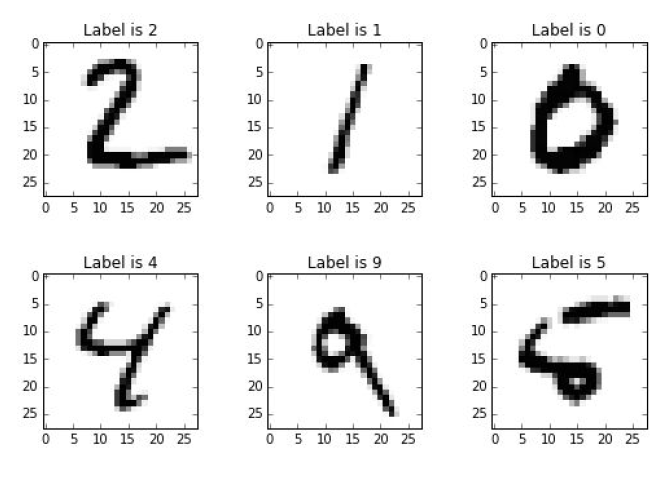
\includegraphics[width=\linewidth]{pics/problem.png}
%     \caption{\label{fig:digit-classification} Digit Classification Problem}
% \end{figure}

\begin{lstlisting}[language=Python]
    # Load the package to plot the data
    import matplotlib.pyplot as mpp

    # Plot the data
    observation = data[0].split(',') # break down observation number 0 (comma is used to identify each element).
    image = np.asfarray(observation[1:]).reshape((28,28)) # take all the elements starting from the element 1 
    # (exclude element number 0, that corresponds to the label) and reshape them as an array with dimension 28 by 28.
    mpp.imshow(image, cmap='Blues', interpolation='None') # show the plot of this array using blue pallete.

    # Save an observation of the data as an input to work with.
    input = np.array(np.asfarray(observation[1:]), ndmin=2).T # save necessary elements in a vertical vector shape.
\end{lstlisting}


\subsection{Fitting the structure of the NN to the Data}

After inspecting the data, we can conclude that the structure in Figure \ref{fig:nn-schema} with 3-5-2 nodes is probably not optimal and therefore should be updated in order to fit the data we have and peculiarities of the classification problem: 

\begin{itemize}
    \item For each observation we have 784 elements as an input (label element is excluded). Accordingly, instead of 3 input nodes we should better have 784.
    \item Similarly, as we have 10 different options for the outcome (handwritten numbers are labeled from from 0 to 9) the number of output nodes should be 10 instead of 2. 
    \item We also change the number of hidden nodes from 5 to 90. Such a number has been assigned based on some proportionality assumptions which will be checked later: 90 is 9 times higher than 10 and approximately 9 times smaller than 784.
\end{itemize}

As we have new structure of the NN we should reassign the weights - now the size of each weight matrix will increase as we have more nodes in each layer.

\begin{lstlisting}[language=Python]
    # Determine the new structure of the NN.
    i_n = 784
    h_n = 90
    o_n = 10
    
    # Determine the weights.
    w_i_h = np.random.rand(h_n, i_n)
    w_h_o = np.random.rand(o_n, h_n)
\end{lstlisting}

So far we have not used the first element of our observation - the label. It will be necessary to compare the predictions of the NN to the real state of the world and to train the NN to make correct predictions. The target should therefore have the same shape as the output layer of the NN, so that they could be comparable. We can represent the label as a vector of n binary (0 or 1) elements (n corresponds to the number of nodes in the output layer). There should be only one element equal to 1 and the position of this element should correspond to the index number of the label we want to predict.

\begin{lstlisting}[language=Python]
    # Create target array.
    target = np.array(np.zeros(o_n), ndmin=2).T
    # int() method returns an integer object
    # from any number or string.
    target[int(observation[0])] = 1 

    # Inspect how the target looks like (remember that the label of observations is 5).
    target

    # Show the sizes of matrices of weights, input and target vectors.
    w_i_h.shape, input.shape, w_h_o.shape, target.shape
\end{lstlisting}

\begin{lstlisting}
((90, 784), (784, 1), (10, 90), (10, 1))
\end{lstlisting}

\subsection{Feedforwarding}

Once we have the structure of the NN updated for the specific task of classifying the numbers depicted on the images, we can run our network in order to get the first predictions that will be represented by a vector of 10 elements. This vector in its turn can be compared to the target.

To run the NN, i.e. to feed forward our input data in order to get some predictions, we should follow certain steps:

\begin{enumerate}
    \item Multiply an input vector by a matrix of weights that connects it with the next layer;
    \item Transform the result using activation function;
    \item Use the output obtained in the 2nd step as an input vector for the next layer.
\end{enumerate}

A sequence of this steps should be repeated n-1 times (where n corresponds to the number of layers). The output of the previous layer will always be the input vector for the next layer. In our case the procedure will happen twice.

In the Figures \ref{fig:multiplication} and \ref{fig:activation}, you can see the procedure necessary to obtain the output of the hidden layer. The result of matrix multiplication here is called Hidden\_Input. Result of the transformation of Hidden\_Input through activation function is called Hidden\_Output.

This output will be used as the input vector that should be multiplied by the next weight matrix and transformed through activation function in order to calculate the final output of the NN. If our NN would have more than one hidden layer, the procedure would be repeated more times.

\begin{figure}[H]
    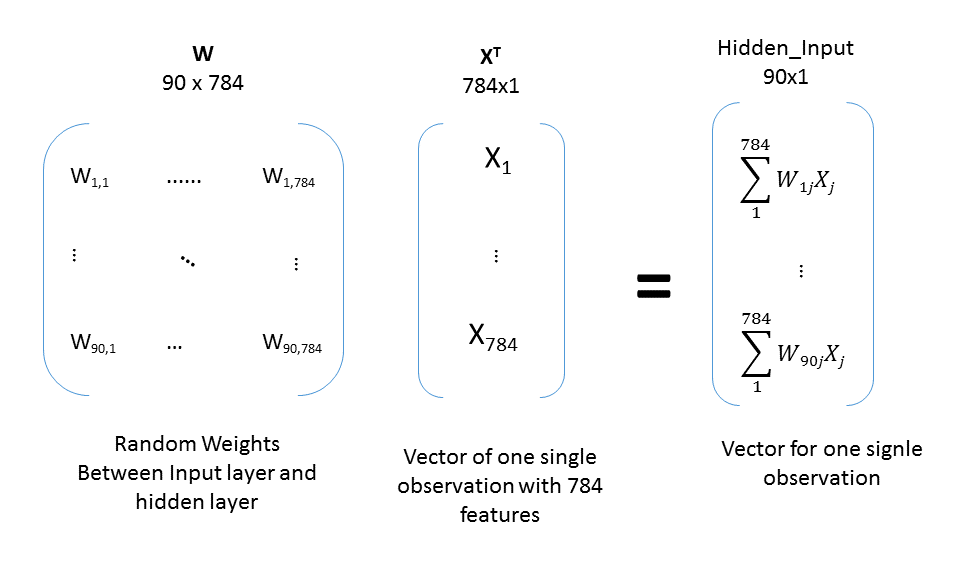
\includegraphics[width=\linewidth]{pics/multiplication.png}
    \caption{\label{fig:multiplication} How Weights Work}
\end{figure}

\begin{figure}[H]
    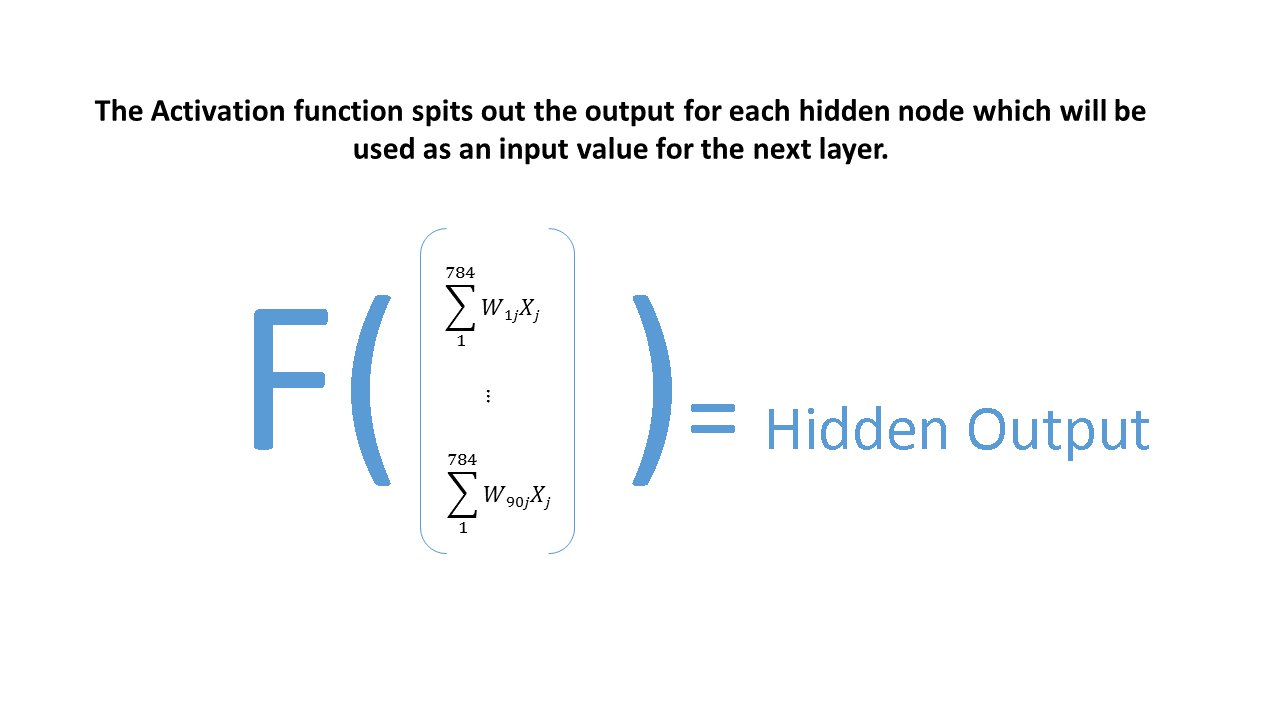
\includegraphics[width=\linewidth]{pics/activation.jpg}
    \caption{\label{fig:activation} How Activation Works}
\end{figure}

Below you can see the code implementation of all the steps for all layers of the NN.

\begin{lstlisting}[language=Python]
    # Calculate the output of hidden and output layers of our NN.
    # dot() performs matrix multiplication; "h_input" stands for "Hidden_Input".
    h_input = np.dot(w_i_h, input) 
    # "Hidden_Output" - result after activation function.
    h_output = sigmoid(h_input) 
    # "Output_Input" - input used for the next layer.
    o_input = np.dot(w_h_o, h_output)
    # "Output_Output" - final output of the NN.
    o_output = sigmoid(o_input)

    # Print output to the screen
    o_output 
\end{lstlisting}

\begin{lstlisting}
    array([[ 1.],
    [ 1.],
    [ 1.],
    [ 1.],
    [ 1.],
    [ 1.],
    [ 1.],
    [ 1.],
    [ 1.],
    [ 1.]])
\end{lstlisting}

\subsection{Good Practices on Data Treatment}


\section{Deep Learning with Keras}
\label{sec:keras}
We are now going to reimplement the previous neural network with the Keras framework. Keras is an open source neural network library written in Python. It has the advantage of abstracting most of the boiler-plate code one needs to write when implementing a neural net only with a linear algebra library. Thus, it is suitable to fast prototyping and experimentation.

It's important you make sure you have the required libraries installed for it to work. We will make use of three main libraries and their dependencies, which will be automatically installed.

If you are using Anconda's Python distribution, we advise you to run \lstinline{conda install keras pandas numpy} on the terminal. 
Otherwise, using the \lstinline{pip} package manager should also do the trick.
Run \lstinline{pip install keras pandas numpy} on the terminal.

The version of Python that will be used throughout this notebook is Python 3.6.4 from Anaconda's distribution. You can check your version of Python by executing the cell below.

\begin{lstlisting}[language=Python]
    import numpy as np
    from keras.models import Sequential
    from keras.layers import Dense
    from keras.utils import np_utils
    
    import pandas as pd
\end{lstlisting}

\subsection{Load the data}

To load the data, we will use the very handy pandas' \lstinline{read_csv} function. It frees us from the burden of parsing the text file.

\begin{lstlisting}[language=Python]
    names = ["y"] + list(range(1,785))
    df = pd.read_csv("data/mnist_train.csv", 
                    names=names)

    df_test = pd.read_csv("data/mnist_test.csv", 
                        names=names)

    df_test.head()
\end{lstlisting}

Next we separate labels from features in both train and test set and transform them from dataframes to numpy arrays, which are better suited for modeling.

\begin{lstlisting}[language=Python]
y_train = df['y'].values
X_train = df.iloc[:, 1:].values/255*0.99+0.01

y_test = df_test['y'].values
X_test = df_test.iloc[:, 1:].values/255*0.99+0.01

[y_train, y_test, X_train, X_test]
\end{lstlisting}

We now check if the shape of the arrays correspond to the expected. In fact, the shape is correct. We have 60 thousand observations in the train set and 10 thousand in the test set.

\begin{lstlisting}[language=Python]
[y_train.shape, X_train.shape, y_test.shape, X_test.shape]
\end{lstlisting}

Before defining the model, one extra step is necessary: transform the labels so they are one-hot encoded. One-hot encoding a vector means transforming it into a matrix of ones and zeroes only with as many columns as the number of different values in the vector. In the specific case, the label vector becomes a ten-column array, each column representing one digit. If the label of the observation is 2, it will have zeroes in columns expect in the third column, which will have a one. The number of rows remains the same. with the same number of rows as before.

\begin{lstlisting}[language=Python]
y_train = np_utils.to_categorical(y_train)
y_test = np_utils.to_categorical(y_test)

[y_test.shape, y_train.shape]
\end{lstlisting}

\subsection{Model}

\subsubsection{Define the model}

We finally come to the most important part. We will accomplish the task of building the neural network with only eight lines of code.

The model in question consists of one input, one hidden and one output layer. The activation function of the hidden layer is a ReLU. And we use as the optimizer Stochastic Gradient Descent. 

Keras makes it very simple to add new layers. One needs only to call the `add` method on the model and pass the layer with its specifications. As you can see, the number of inputs needs to be specified only in the first layer. Keras infers the input number of a layer by looking at the number of outputs of its predecessor.

For this neural network, we will only use dense layers, which are layers with all nodes fully connected to each other. Keras, however, allows you to arbitrarily build your neural networks by providing different types of layers, such as convolutional and pooling layers.

\begin{lstlisting}[language=Python]
    def baseline_model(num_hidden_n, num_pixels, num_classes, optimizer):
        model = Sequential()
        model.add(Dense(num_hidden_n, input_dim=num_pixels, kernel_initializer='normal', activation='relu'))
        model.add(Dense(num_classes, kernel_initializer='normal', activation='softmax'))
        
        # Compile model
        model.compile(loss='categorical_crossentropy', 
                    optimizer=optimizer,
                    metrics=['accuracy'])
        return model
\end{lstlisting}

\subsubsection{Instantiate the model}

Having defined the structure of the model, we can now instantiate a concrete version of it by picking the relevant parameters and calling the function that returns the model object.

Here we have chosen the hidden layers to have 90 nodes, while input and output layers have 784 and 10 nodes respectively. 

\begin{lstlisting}[language=Python]
    num_pixels, num_hidden_n, num_classes = 784, 90, 10
    optimizer = 'sgd'
    
    model = baseline_model(num_hidden_n, num_pixels, num_classes, optimizer)
\end{lstlisting}

\subsubsection{Train and evaluate the model}

With the model instantiated, we can finally call the fit method on it using the data set we prepared before.

After training the model we evaluate its performance by looking at its accuracy.

\begin{lstlisting}[language=Python]
    model.fit(X_train,
        y_train, 
        epochs=5,
        batch_size=200,
        verbose=2)
    scores = model.evaluate(X_test, y_test, verbose=0)
    print("Baseline Error: %.2f%%" % (100-scores[1]*100))
\end{lstlisting}

\begin{lstlisting}
    Epoch 1/5
    - 2s - loss: 1.9537 - acc: 0.5054
   Epoch 2/5
    - 2s - loss: 1.1453 - acc: 0.7680
   Epoch 3/5
    - 2s - loss: 0.7509 - acc: 0.8296
   Epoch 4/5
    - 2s - loss: 0.5942 - acc: 0.8552
   Epoch 5/5
    - 2s - loss: 0.5129 - acc: 0.8706
   Baseline Error: 11.96%
\end{lstlisting}

The error rate does not seem very good. Maybe we could try a different optimizer. We will instantiate and fit the model again with the RMSprop optimization algorithm. By using Keras, the only thing you need to do is to pass a different argument to the model.

\begin{lstlisting}[language=Python]
    model = baseline_model(num_hidden_n,
        num_pixels,
        num_classes,
        optimizer = "rmsprop")

    model.fit(X_train,
    y_train, 
    epochs=5,
    batch_size=200,
    verbose=2)
    scores = model.evaluate(X_test, y_test, verbose=0)
    print("Baseline Error: %.2f%%" % (100-scores[1]*100))
\end{lstlisting}

\begin{lstlisting}
    Epoch 1/5
    - 2s - loss: 0.4963 - acc: 0.8723
   Epoch 2/5
    - 2s - loss: 0.2401 - acc: 0.9306
   Epoch 3/5
    - 2s - loss: 0.1828 - acc: 0.9477
   Epoch 4/5
    - 2s - loss: 0.1466 - acc: 0.9581
   Epoch 5/5
    - 2s - loss: 0.1223 - acc: 0.9640
   Baseline Error: 3.54%   
\end{lstlisting}

\subsubsection{Save the model}

Once trained, you might want to use the model in the future. You can do so by saving it to a file for later use. Keras comes equipped with the `save` method, which allows you to easily save your trained model to the disk.

We are going to save the model into a file called `model.h5` and delete it from memory.

\begin{lstlisting}[language=Python]
    model.save("model.h5")
    del model    
\end{lstlisting}

Then we load the model from the file we just created and evaluate it again to make sure that during the saving process, the model hasn't been corrupted. The base line error is the same: the model has been successfully saved and can be shared with third-parties. 

\begin{lstlisting}[language=Python]
    from keras.models import load_model

    model2 = load_model("model.h5")
    
    scores2 = model2.evaluate(X_test, y_test, verbose=0)
    print("Baseline Error: %.2f%%" % (100-scores2[1]*100))    
\end{lstlisting}


% BibTeX users please use one of
%\bibliographystyle{spbasic}    % basic style, author-year citations
%\bibliographystyle{spmpsci}     % mathematics and physical sciences
%\bibliographystyle{spphys}     % APS-like style for physics
% \bibliographystyle{plain}
% \bibliography{references}       % name your BibTeX data base

\printbibliography
\end{document}
% end of file template.tex

